% ---------- chapters/results.tex ----------
\chapter{Results}\label{ch:results}

\section{Training Dynamics}

Figure~\ref{fig:train_loss} traces the negative‑log‑likelihood over 55
epochs.  Loss falls from roughly 6.3 to 1.0 without signs of over‑fitting,
confirming that streaming the dataset and saving checkpoints every epoch is
sufficient for stable convergence.

\begin{figure}[!ht]
    \centering
    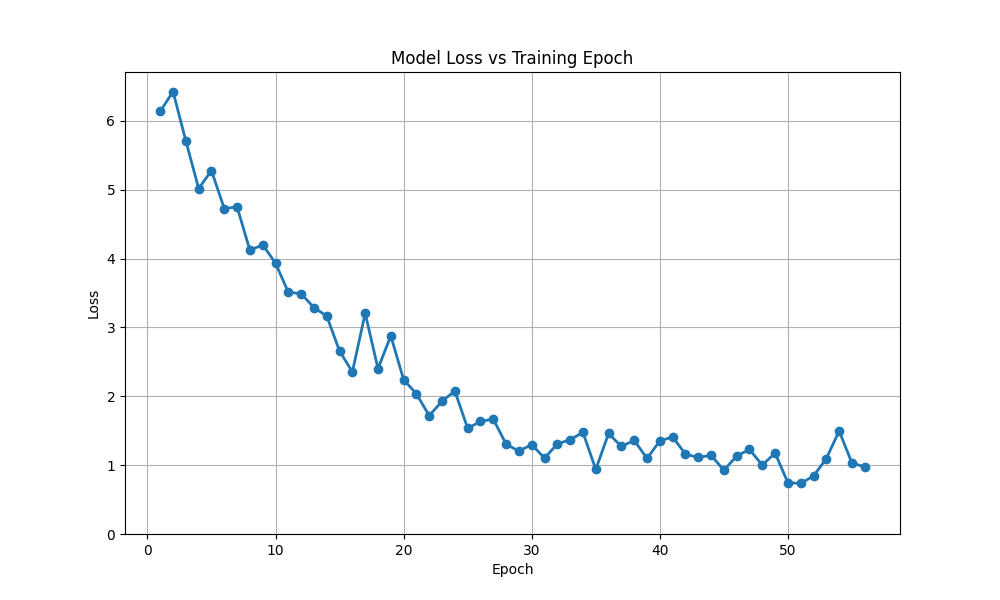
\includegraphics[width=0.8\textwidth]{figs/training_loss_plot.png}
    \caption{Training loss (NLL) versus epoch for the latent‑recurrence model.}
    \label{fig:train_loss}
\end{figure}

\section{Effect of Recurrence Depth}

We evaluated the same checkpoint at seven recurrence depths
\(r\in\{1,2,4,6,8,12,24\}\).
Average cross‑entropy on 500 held‑out samples is visualised in
Figure~\ref{fig:rec_loss} and summarised numerically in
Table~\ref{tab:rec_results}.

\begin{figure}[!ht]
    \centering
    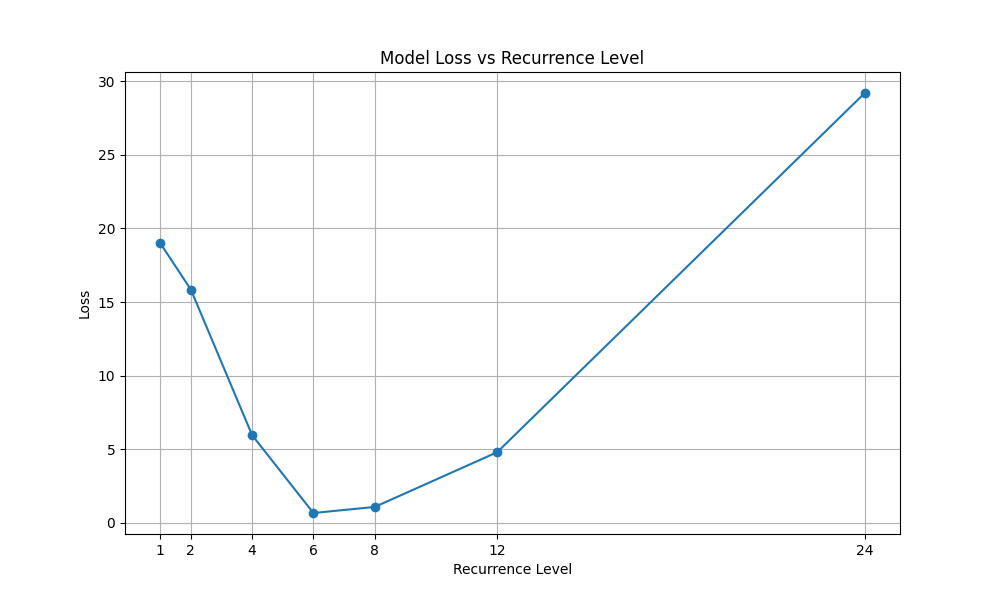
\includegraphics[width=0.8\textwidth]{figs/recurrence_plot.png}
    \caption{Validation loss as a function of recurrence depth \(r\).}
    \label{fig:rec_loss}
\end{figure}

% ---------- tables/recurrence_results.tex ----------
\begin{table}[!ht]
\centering
\begin{tabular}{|c|c|}
\hline
\textbf{Recurrence \(r\)} & \textbf{Average Loss} \\ \hline
1  & 19.1 \\
2  & 15.8 \\
4  &  6.1 \\
6  &  0.6 \\
8  &  0.9 \\
12 &  4.8 \\
24 & 29.4 \\ \hline
\end{tabular}
\caption{Cross‑entropy loss at different recurrence depths (latent‑recurrence model).}
\label{tab:rec_results}
\end{table}


\paragraph{Observations}

\begin{itemize}
    \item Loss decreases steeply up to \(r=6\) where it reaches a minimum
          of 0.6.  This confirms that a modest amount of latent looping
          can dramatically sharpen the distribution without any extra
          parameters.
    \item Beyond \(r=8\) the benefit reverses; at \(r=24\) loss is higher
          than the single‑pass baseline, indicating accumulated numerical
          noise or over‑correction.
    \item With the current implementation, the sweet‑spot
          for compute‑to‑quality trade‑off lies in the range
          \(r=4\)–\(6\).
\end{itemize}
